\documentclass{../TexTemplate/myslide}
\usepackage[slide,table,python]{../TexTemplate/mypackage}
\hypersetup{colorlinks=true,linkcolor=black,urlcolor=blue}
\usepackage{xcolor}

\renewcommand{\thefootnote}{\fnsymbol{footnote}}

\title[ToolsSeminar]{Tools Seminar}
\subtitle{Week 6 - Scientific Computing}
\author[chhzh123]{Hongzheng~Chen}
\date[Mar 22, 2020]{Mar 22, 2020}

\begin{document}

\begin{frame}
\titlepage
\end{frame}

\begin{frame}
\tableofcontents
\end{frame}

\section{Introduction}
\begin{frame}
\sectionpage
\end{frame}

\begin{frame}{Scientific Computation}
Mostly involve applied mathematics and computational mathematics
\begin{itemize}
	\item Quantitative finance (stock)
	\item Physical simulation (fluid, illumination, cloth $\to$ \href{https://www.youtube.com/watch?v=EhDr3Rs5fTU}{CG})
	% http://graphics.stanford.edu/courses/cs348c/
	\item Computational biology (gene)
	\item Molecular dynamics (protein)
	\item Ocean circulation
	\item Weather/Climate prediction
\end{itemize}
\end{frame}

\begin{frame}{Scientific Computation}
Mostly involve applied mathematics and computational mathematics
\begin{itemize}
	\item Astronomy (1st \href{https://www.zhihu.com/question/318763133/answer/647517757}{black hole} photo $\to$ digital image processing)
	% Katherine L. Bouman, Extreme Imaging via Physical Model Inversion: Seeing Around Corners and Imaging Black Holes
	\begin{figure}[H]
	\centering
	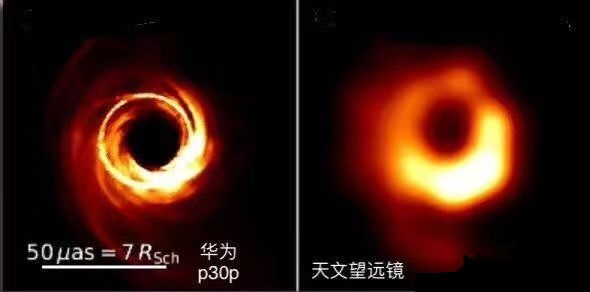
\includegraphics[width=0.6\linewidth]{fig/blackhole.jpg}
	\caption*{\scriptsize Fig source: Weibo}
	\end{figure}
	\[\hat{\vx}=\argmin_{\vx}[(f(\vx)-\vy)^\T\mathbf{R}^{-1}(f(\vx)-\vy)+(\vx-\vmu)^\T\Lambda^{-1}(\vx-\vmu)]\;,\]
	where $\hat{\vx}$ is the photo needed to be reconstructed.
\end{itemize}
\end{frame}

\begin{frame}[fragile]{Scientific Computation}
Mostly involve applied mathematics and computational mathematics
\begin{itemize}
	\item Epidemics (\href{https://www.zhihu.com/question/367466399/answer/982597090}{COVID-19} $\to$ SEIR model)
\end{itemize}
\begin{center}
\small
\begin{tikzcd}
\text{Susceptible} (S)\arrow[r, "\beta"]
& \text{Exposed} (E)\arrow[r, "\sigma"]
& \text{Infectious} (I)\arrow[r, "\gamma"]
& \text{Recovered} (R)
\end{tikzcd}
\end{center}
\[\begin{cases}
\frac{\diff S}{\diff t}=\mu N-\nu S-\frac{\beta SI}{N}\\
\frac{\diff E}{\diff t}=\frac{\beta S I}{N} - vE-\sigma E\\
\frac{\diff I}{\diff t}=\sigma E-\gamma I-\nu I\\
\frac{\diff R}{\diff t}=\gamma I-\nu R
\end{cases}\]
\pause
* \href{http://www.nscc-gz.cn/}{Supercomputing} enables more complex applications to be done
\end{frame}

\begin{frame}{Features of Scientific Computation}
Gap between sci. comp. \& real computer:
\[\begin{array}{ccc}
\textbf{Real Computer} &  & \textbf{Sci. Comp.}\\
\text{discrete} & \iff & \text{continuous}\\
\text{integer} & \iff & \textbf{\textcolor{red}{real numbers}}
\end{array}\]
\pause
\href{http://754r.ucbtest.org/standards/754xml.html}{IEEE 754 binary floating point standard}
\[(-1)^s\times m\times 2^{e-127}\]
Be careful of the \textbf{roundoff error}!\\
Try $5.2-5$ in Python
\end{frame}

\begin{frame}[fragile]{Features of Scientific Computation}
Most of them are \textbf{matrix computation}! (GEMM)\\
e.g. gradient descent, convolution, Gauss-Seidel, $\ldots$
\[c_{ij}=\sum_k a_{ik}b_{kj}\]
\begin{lstlisting}[language=c++]
for (int i = 0; i < M; i++)
    for (int j = 0; j < N; j++)
        for (int k = 0; k < K; k++)
            C[i][j] += A[i][k] * B[k][j];
\end{lstlisting}
\pause
Time complexity: $O(n^3)$, is it true?\\
\pause
Optimistically regard the memory as plain, but $\ldots$
\end{frame}

\begin{frame}{Memory Hierarchy}
Recommend to read \href{https://csapp.cs.cmu.edu/}{CSAPP}!
\begin{figure}
\centering
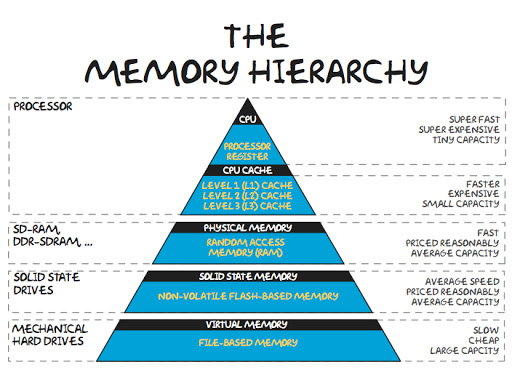
\includegraphics[width=0.7\linewidth]{fig/memory_hierarchy.jpg}
\caption*{\scriptsize Fig source: \url{http://computerscience.chemeketa.edu/cs160Reader/ComputerArchitecture/MemoryHeirarchy.html}}
\end{figure}
\end{frame}

\begin{frame}[fragile]{Temporal \& Spatial Locality}
Recommend to read \href{https://csapp.cs.cmu.edu/}{CSAPP}!
\begin{columns}
\begin{column}{0.55\linewidth}
\begin{figure}
\centering
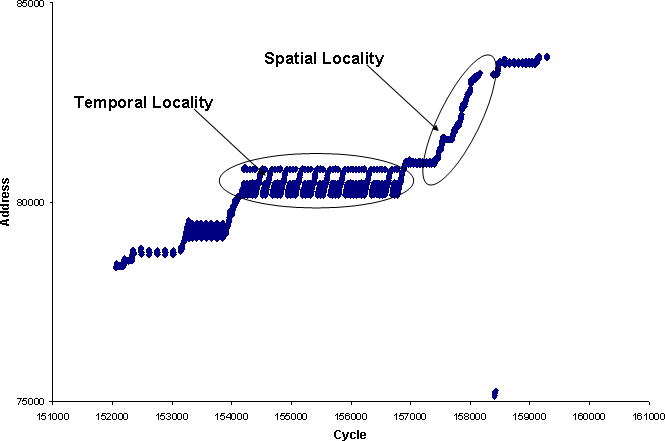
\includegraphics[width=\linewidth]{fig/locality.png}
\caption*{\scriptsize Fig source: \url{https://stackoverflow.com/a/49325155}}
\end{figure}
\end{column}
\begin{column}{0.45\linewidth}
\begin{lstlisting}[language=c++]
int sum = 0;
for (int i = 0; i < 10; ++i)
    sum = sum + a[i];
\end{lstlisting}
\end{column}
\end{columns}
\end{frame}

\begin{frame}[fragile]{Back to GEMM}
You should know how to store a 2D array in computer memory
\[\bmat{1 & 2\\3 & 4}\]
\begin{itemize}
	\item Row-major: \verb'{{1,2},{3,4}}' (C/C++)
	\item Column-major: \verb'{{1,3},{2,4}}' (Matlab)
\end{itemize}
% https://en.wikipedia.org/wiki/Row-_and_column-major_order
\end{frame}

\begin{frame}[fragile]{Back to GEMM}
\begin{lstlisting}[language=c++]
for (int i = 0; i < M; i++)
    for (int j = 0; j < N; j++)
        for (int k = 0; k < K; k++)
            C[i][j] += A[i][k] * B[k][j];
\end{lstlisting}
\begin{figure}
\centering
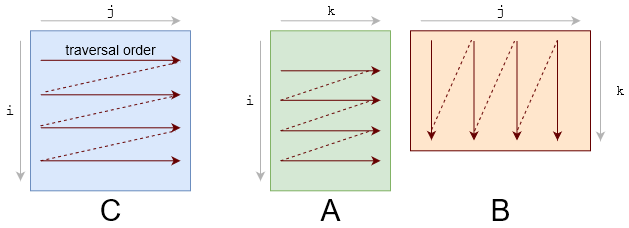
\includegraphics[width=0.8\linewidth]{fig/gemm.png}
\caption*{\scriptsize Fig source: \href{https://sahnimanas.github.io/post/anatomy-of-a-high-performance-convolution/img/naive-traversal.svg}{Sahnimanas}}
\end{figure}
\end{frame}

\begin{frame}{Back to GEMM}
\begin{figure}
\centering
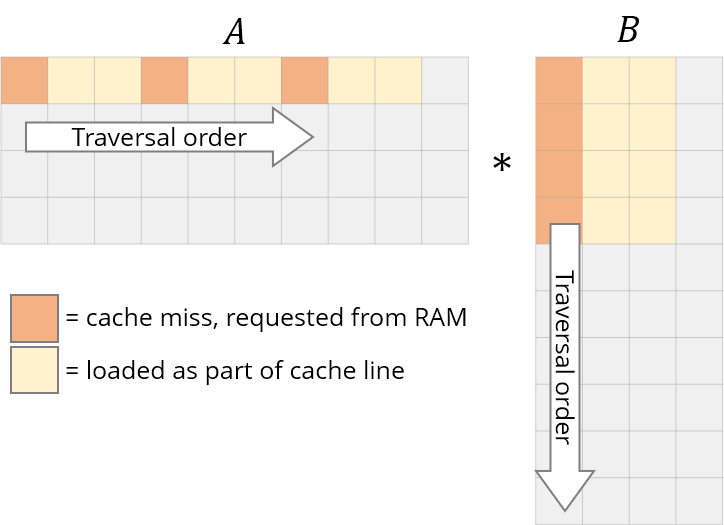
\includegraphics[width=0.8\linewidth]{fig/cache-pollution.png}
\caption*{\scriptsize Fig source: \href{https://sahnimanas.github.io/post/anatomy-of-a-high-performance-convolution/img/cache-pollution.png}{Sahnimanas}}
\end{figure}
\end{frame}

\begin{frame}[fragile]{Back to GEMM}
\begin{lstlisting}[language=c++]
for (int i = 0; i < M; i++)
    for (int k = 0; k < K; k++) // reordering
        for (int j = 0; j < N; j++)
            C[i][j] += A[i][k] * B[k][j];
\end{lstlisting}
\begin{figure}
\centering
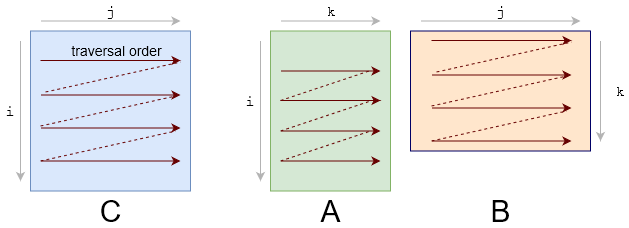
\includegraphics[width=0.75\linewidth]{fig/reordering.png}
\caption*{\scriptsize Fig source: \href{https://sahnimanas.github.io/post/anatomy-of-a-high-performance-convolution/img/reordered.svg}{Sahnimanas}}
\end{figure}
Data organization greatly affects performance, more than 10x speedup!!!
\end{frame}

\begin{frame}{Scientific Computation Requirements}
\begin{itemize}
	\item Calculus
	\item Linear Algebra
	\item Differential Equations (pde / ode)
	\item Convex Optimization
	\item Numerical Computing
	\item Computer System \& Architecture
	\item Parallel Computing
	\item $\cdots$
\end{itemize}
\pause
Thankfully, we have lots of tools to support sci. comp.
\end{frame}

\section{Package Management}
\begin{frame}
\sectionpage
\end{frame}

\begin{frame}{Why we need package management?}
Installing third-party library for \underline{C/C++} is very awkward (boost, OpenGL, $\ldots$)
\begin{enumerate}[<+->]
	\item Download source code with magic version from some unknown webpages
	\item Put the code in some system folder that is hard to find
	\item Compile the library
	\item If gcc/make version not correct, go back to 1
	\item If dependency files not found, go back to 1
	\item Successfully compiled but the package not found, go back to 2
	\item Run the package but get runtime error, go back to 1
	\item $\cdots$
\end{enumerate}
\pause
Thus, we need tools to help us \textbf{build, manage, upgrade, remove} different kinds of packages
\end{frame}

\begin{frame}[fragile]{Package Management}
Fortunately, \underline{Python} has powerful package management tools!
\begin{itemize}
	\item Windows: \href{https://www.anaconda.com/}{Anaconda} (conda)
	\begin{itemize}
		\item The complete data science platform
		\item If you want to use your own GPU for deep learning in the future, you should install
		\item Remember to change the mirror to \href{https://mirror.tuna.tsinghua.edu.cn/help/anaconda/}{Tsinghua}, or downloading will be very slow
	\end{itemize}
	\item Linux: \href{https://pip.pypa.io/en/stable/}{pip} (The Python Package Installer)
	\begin{itemize}
		\item Be careful of your Python version (2 or 3)
		\item \verb'sudo apt install python-pip'
		\item \verb'sudo apt install python3-venv python3-pip'
		\item \verb'pip3 -V'
	\end{itemize}
\end{itemize}
\end{frame}

\begin{frame}[fragile]{Package Management}
\begin{itemize}
	\item \verb'pip install ...'
	\item \verb'pip install --upgrade ...'
	\item \verb'pip uninstall ...'
	\item \verb'pip list'
\end{itemize}
\end{frame}

\begin{frame}[fragile]{Environment Management}
If you need to regularly change Python version, please create a \href{https://virtualenv.pypa.io/en/latest/}{virtual environment}!\\
\verb'pip3 install virtualenv'
% https://tecadmin.net/use-virtualenv-with-python3/
\begin{itemize}
	\item \verb'which python3'
	\item \verb'virtualenv -p /usr/bin/python3 mypy3'
	\item \verb'source mypy3/bin/activate'
	\begin{itemize}
		\item Then you can directly call Python 3 by \verb'python'
	\end{itemize}
	\item \verb'deactivate'
\end{itemize}
conda has inherent environment management tool:
\begin{itemize}
	\item \verb'conda create -n your_env_name python=your_py_version'
	\item \verb'activate env_name'
	\item \verb'deactivate'
\end{itemize}
\end{frame}

\begin{frame}[fragile]{Environment Management}
\href{https://dev.to/bhupesh/pipreqs-automatically-generate-python-dependencies-30nl}{pipreqs}: Automatically generate python dependencies
\begin{itemize}
	\item \verb'pip3 install pipreqs'
	\item \verb'pipreqs /<your_project_path>/'
	\item \verb'pip3 install -r requirements.txt'
\end{itemize}
\end{frame}

\begin{frame}[fragile]{Jupyter Notebook}
\href{https://jupyter.org/}{Jupyter notebook}: A extremely powerful web-based interactive interface
\begin{itemize}
	\item \verb'pip3 install notebook'
	\item \verb'jupyter notebook'
	\begin{itemize}
		\item You should first \verb'cd' to the folder you want to open
	\end{itemize}
	\item Code, data, figure, notes (Markdown)
	\item Also valid on Github and VS Code
	\item Next-generation notebook: \href{https://jupyter.org/}{Jupyter Lab}
\end{itemize}
\end{frame}

\section{SciPy}
\begin{frame}
\sectionpage
\end{frame}

\begin{frame}[fragile]{SciPy}
\href{https://www.scipy.org/}{SciPy}: a Python-based ecosystem of open-source software for mathematics, science, and engineering
\begin{itemize}
	\item \underline{NumPy}: Base N-dimensional array package
	\item SciPy library: Fundamental library for scientific computing (FFT, signal, opt, $\ldots$)
	\item \underline{Matplotlib}: Comprehensive 2-D plotting
	\item IPython: Enhanced interactive console
	\item SymPy: Symbolic mathematics
	\item \underline{pandas}: Data structures \& analysis
\end{itemize}
* Anaconda must contain scipy package\\
For Linux, install by \verb'pip3 install scipy'
\end{frame}

\begin{frame}[fragile]{Numpy}
\href{https://numpy.org/}{Numpy}: \verb'pip3 install numpy' 
\begin{itemize}
	\item A powerful N-dimensional array object
	\item Sophisticated (broadcasting) functions
	\item Tools for integrating C/C++ and Fortran code (core part of numpy is written in C)
	\begin{itemize}
		\item Integrated with \href{https://software.intel.com/en-us/mkl}{Intel Math Kernel Library (MKL)}, thus is super fast!
	\end{itemize}
	\item Useful linear algebra, Fourier transform, and random number capabilities
	\item Indexing, slicing, and iterating functions the same way as in Python
\end{itemize}
Tutorial: \url{https://docs.scipy.org/doc/numpy/user/quickstart.html}
\end{frame}

\begin{frame}[fragile]{The Basics}
\verb'import numpy as np'
\begin{itemize}
	\item \verb'np.array([[1,2,3],[4,5,6]])'
	\item \verb'a.shape', \verb'a.size', \verb'a.ndim'
	\begin{itemize}
		\item Be careful of the shape of \verb'np.array([1,2,3])'
		\item Differentiate between \verb'(3,)' and \verb'(3,1)'
	\end{itemize}
	\item \verb'a.dtype'
	\begin{itemize}
		\item Python is strong-typed
		\item \verb'a.astype(np.float64)'
	\end{itemize}
	\item \verb'a.reshape((3,2))'
	\begin{itemize}
		\item Input a tuple! Not transpose! Return a new array!
		\item Distinguish with \verb'a.T'
		\item \verb'a.resize' is inplace
	\end{itemize}
\end{itemize}
\end{frame}

\begin{frame}[fragile]{Array Creation}
\begin{itemize}
	\item \verb'np.zeros((3,4))'
	\item \verb'np.ones((3,4))'
	\item \verb'np.arange(1,10,1)' $[a,b)$
	\item \verb'np.linspace(0,1,10)'
	\item \verb'np.random.random((3,4))'
\end{itemize}
\end{frame}

\begin{frame}[fragile]{Stacking}
\begin{itemize}
	\item \verb'np.column_stack((a,b))', \verb'np.hstack'
	\item \verb'np.row_stack((a,b))', \verb'np.vstack'
\end{itemize}
\end{frame}

\begin{frame}[fragile]{Basic Operations}
Arithmetic operations are \textbf{element-wise} if both are arrays of same size!
\begin{itemize}
	\item \verb'+,-,*,/,**'
	\item \verb'<,>,=='
\end{itemize}
\end{frame}

\begin{frame}[fragile]{Broadcasting}
\href{https://docs.scipy.org/doc/numpy/user/basics.broadcasting.html}{Broadcasting rules}: Examine if two dimensions are compatible
\begin{itemize}
	\item they are equal, or
	\item one of them is $1$
\end{itemize}
\begin{lstlisting}
Image  (3d array): 256 x 256 x 3
Scale  (1d array):               3
Result (3d array): 256 x 256 x 3

A      (2d array):  5 x 4
B      (1d array):       1
Result (2d array):  5 x 4

A      (4d array):  8 x 1 x 6 x 1
B      (3d array):       7 x 1 x 5
Result (4d array):  8 x 7 x 6 x 5
\end{lstlisting}
\begin{itemize}
	\item \verb'+,-,*,/,**'\qquad \verb'<,>,=='
	\item \verb'np.sin', \verb'np.exp', \verb'np.sqrt'
\end{itemize}
\end{frame}

\begin{frame}[fragile]{Matrix Product}
Notice: \verb'*' for numpy array is the element-wise or \textbf{Hadamard product}, denoted as
\[(A\circ B)_{ij}=(A)_{ij}(B)_{ij}\]
\bigskip
The true \textbf{matrix product} can be called as shown below
\begin{lstlisting}
>>> a @ b                       # matrix product
>>> a.dot(b)                    # another matrix product
>>> c = np.matrix([[1,2],[3,4]])
>>> c * d                       # also matrix product
\end{lstlisting}
\end{frame}

\begin{frame}[fragile]{Clustering Functions}
Axis: Extremely important! Ref: \url{https://www.sharpsightlabs.com/blog/numpy-axes-explained/}
\begin{figure}
\centering
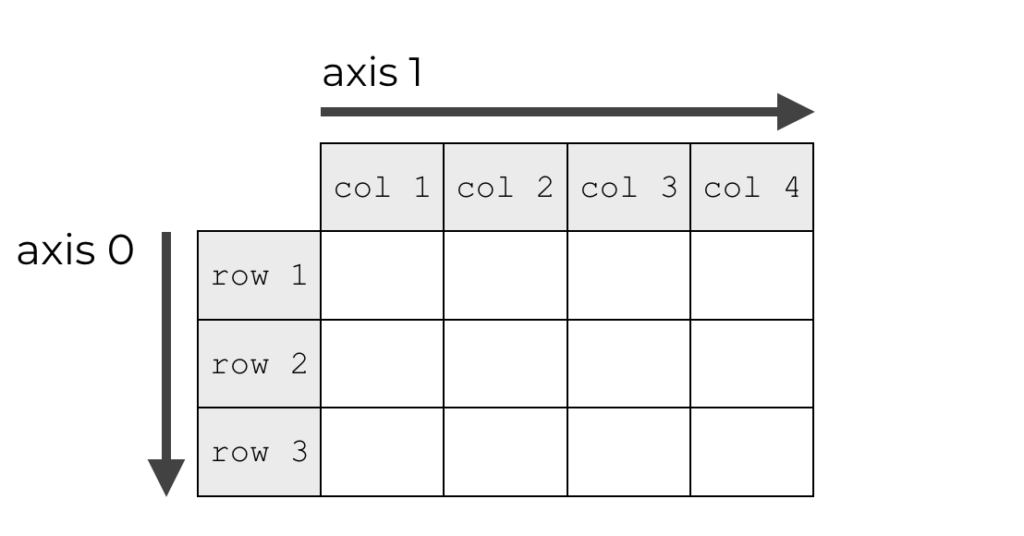
\includegraphics[width=0.8\linewidth]{fig/axis1.png}
\end{figure}
\end{frame}

\begin{frame}[fragile]{Clustering Functions}
Axis: Extremely important! Ref: \url{https://www.sharpsightlabs.com/blog/numpy-axes-explained/}
\begin{figure}
\centering
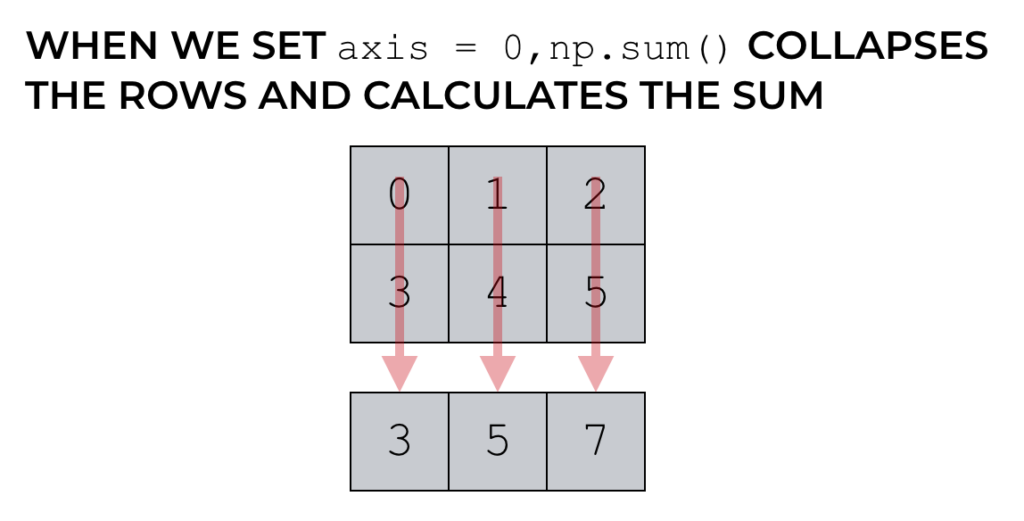
\includegraphics[width=0.8\linewidth]{fig/axis2.png}
\end{figure}
\verb'np.sum(a,axis=0)', \verb'np.mean', \verb'np.min', \verb'np.max', \verb'F.softmax' (pytorch)
\end{frame}

\begin{frame}[fragile]{Indexing \& Slicing}
Basic indexing \& Slicing:
\begin{itemize}
	\item \verb'a[:]', \verb'a[:6:2]', \verb'a[::-1]'
	\item \verb'b[ : , 1:3]', \verb'b[ : , 2]'
\end{itemize}
Fancy indexing: Use array of indices
\begin{itemize}
	\item \verb'a[b]'
	\item \verb'a[a>2]'
	\item Even assignment is allowed, like \verb'a[a>2] = 0'
\end{itemize}
\end{frame}

\begin{frame}[fragile]{Linear Algebra}
\begin{itemize}
	\item \verb'np.eye'
	\item \verb'a.transpose'
	\item \verb'np.linalg.inv(a)'
	\item \verb'np.linalg.trace(a)'
	\item \verb'np.linalg.solve(a,y)'
	\item \verb'np.linalg.eig(a)'
\end{itemize}
\end{frame}

\begin{frame}[fragile]{More About Product Summation}
\verb'np.einsum(equation, *operands)' (Einstein summation convention)
\small
\begin{center}
\begin{tabular}{llll}\hline\hline
Transpose & $c_{ij}=a_{ji}$ & $c_{ij}=a_{ji}$ & \verb'ij->ji' \\
Dot product & $c=\sum_i a_ib_i$ & \qquad\qquad & \qquad\qquad \\
Outer product & $c_{ij}=a_ib_j$ & \qquad\qquad & \qquad\qquad \\
Summation & $c_i=\sum_j a_{ij}$ & \qquad\qquad & \qquad\qquad \\
Trace & $c=\sum_i a_{ii}$ & \qquad\qquad & \qquad\qquad \\
Hadamard product & $c_{ij}=a_{ij}b_{ij}$ & \qquad\qquad & \qquad\qquad \\
Matrix-vector product & $c_i=\sum_jA_{ij}b_j$ & $c_i=a_{ij}b_j$ & \verb'ij,j->i' \\
Matrix-matrix product & $c_{ik}=\sum_ja_{ij}b_{jk}$ & \qquad\qquad & \qquad\qquad \\
Tensor product & $c_{kl}=\sum_i\sum_ja_{ijk}b_{ijl}$ & \qquad\qquad & \qquad\qquad \\
\hline
\end{tabular}
\end{center}
\end{frame}

\begin{frame}[fragile]{More About Product Summation}
\verb'np.einsum(equation, *operands)' (Einstein summation convention)
\small
\begin{center}
\begin{tabular}{llll}\hline\hline
Transpose & $c_{ij}=a_{ji}$ & $c_{ij}=a_{ji}$ & \verb'ij->ji'\\
Dot product & $c=\sum_i a_ib_i$ & $c=a_ib_i$ & \verb'i,i->' or \verb'i,i'\\
Outer product & $c_{ij}=a_ib_j$ & $c_{ij}=a_ib_j$ & \verb'i,j->ij'\\
Summation & $c_i=\sum_j a_{ij}$ & $c_i=a_{ij}$ & \verb'ij->i'\\
Trace & $c=\sum_i a_{ii}$ & $c=a_{ii}$ & \verb'ii'\\
Hadamard product & $c_{ij}=a_{ij}b_{ij}$ & $c_{ij}=a_{ij}b_{ij}$ & \verb'ij,ij->ij'\\
Matrix-vector product & $c_i=\sum_jA_{ij}b_j$ & $c_i=a_{ij}b_j$ & \verb'ij,j->i'\\
Matrix-matrix product & $c_{ik}=\sum_ja_{ij}b_{jk}$ & $c_{ik}=a_{ij}b_{jk}$ & \verb'ij,jk->ik'\\
Tensor product & $c_{kl}=\sum_i\sum_ja_{ijk}b_{ijl}$ & $c_{kl}=a_{ijk}b_{ijl}$ & \verb'ijk,ijl->kl'\\
\hline
\end{tabular}
\end{center}
Easy to write, and very efficient!\\
Ref:
\begin{itemize}
	\item \url{https://stackoverflow.com/a/33641428}
	\item \url{https://zhuanlan.zhihu.com/p/71639781}
\end{itemize}
\end{frame}

\begin{frame}{Some hints for efficient implementation}
\begin{itemize}
	\item Do NOT use naive Python loop!
	\item Think of matrix/tensor representation instead of scalar
	\item Use inherent matrix operators
\end{itemize}
\end{frame}

\section{Math Softwares}
\begin{frame}
\sectionpage
\end{frame}

\begin{frame}{Math Softwares for Scientific Computing}
3M in Mathematics
\begin{itemize}
	\item Matlab: \underline{Numeric} computation, C-like grammar, efficient for engineering
	\item Mathematica: \underline{Symbolic} computation, Wolfram Language, fantastic visualization effect, rich documentation (\textcolor{red}{highly recommended!})
	\item Maple: \underline{Symbolic} computation, few people use now (DONT USE!)
\end{itemize}
* Many computation tasks can be done by Python/\href{https://julia.mit.edu/}{Julia} now, and the importance of Matlab is sharpen.
\end{frame}

\begin{frame}{Installation}
\begin{itemize}
	\item \href{https://software.sysu.edu.cn/matlabhome}{Matlab R2019b} (student version)
	\begin{itemize}
		\item Use the campus Internet to download
	\end{itemize}
	\item \href{https://tiebamma.github.io/InstallTutorial}{Mathematica 12.0}
	\begin{itemize}
		\item \$50 for student version
		\item Online version: \url{https://www.wolframcloud.com/}
	\end{itemize}
\end{itemize}
\end{frame}

\begin{frame}[fragile]{Basic Usage}
Similar to Python's interactive window, but with much more powerful functional support
\begin{itemize}
	\item Type in display mode
	\begin{itemize}
		\item Ctrl+2: square root
		\item Ctrl+4: superscript
		\item Ctrl+/: fraction
	\end{itemize}
	\item \verb'Solve[equ,var]'
	\begin{itemize}
		\item \verb'==' represents equal, \verb'=' means assignment
		\item Symbolic, high-order, parameter, equation systems
		\item \verb'NSolve' for numerical results
		\item \verb'Reduce' for constrained solutions
	\end{itemize}
	\item \verb'D[f]', \verb'Integral[f,var]', \verb'Integral[f,{var,x_min,y_min}]'
	\begin{itemize}
		\item High-order, multiple variables
		\item Display the steps
		% Trace[Integrate[Sin[x]^n,{x,0,Pi/2}],TraceInternal->True]
	\end{itemize}
\end{itemize}
\end{frame}

\begin{frame}[fragile]{Basic Usage}
\begin{itemize}
	\item \verb'Sum[exp,var]'
	\item \verb'Simplify[exp]'
	\item \verb'Plot[f,{x,x_min,x_max}]'
	\begin{itemize}
		\item \verb'ContourPlot', \verb'ListLinePlot', \verb'ParametricPlot'
	\end{itemize}
	\item You can even copy the formulas as \LaTeX
	\item The most powerful thing: Enormous database!
	\item Explore more in
	\begin{itemize}
		\item \url{https://www.wolfram.com/mathematica/}
		\item \url{https://www.zhihu.com/question/27834147}
	\end{itemize}
\end{itemize}
\textbf{* Make the best of the manual!}
\end{frame}

\section{Summary}
\begin{frame}
\sectionpage
\end{frame}

\begin{frame}{Summary}
\begin{itemize}
	\item Introduction
	\item Package management: pip, Anaconda
	\item Useful tools: virtualenv, pipreqs, jupyter notebook
	\item Numpy: fancy indexing, broadcasting, linear algebra
	\item Math software: Matlab, Mathematica
\end{itemize}
* We won't cover Python's OOP \& stl in the seminar, but please be familiar with it
\end{frame}

\end{document}